\documentclass[12pt, a4paper, oneside]{ctexart}
\usepackage{amsmath, amsthm, amssymb, bm, graphicx, hyperref, mathrsfs,subfigure,float,adjustbox}

\title{\textbf{机器学习 第二周作业}}
\author{樊泽羲 2200010816}
\date{\today}
\linespread{1.5}
\newcounter{problemname}
\newenvironment{problem}{\stepcounter{problemname}\par\noindent\textbf{题目\arabic{problemname}. }}{\\\par}
\newenvironment{solution}{\par\noindent\textbf{解答. }}{\\\par}
\newenvironment{note}{\par\noindent\textbf{题目\arabic{problemname}的注记. }}{\\\par}

\begin{document}

\maketitle

\begin{problem}
    验证感知机为什么不能表示XOR
\end{problem}
\begin{figure}[H]% 插入一张图片,H表示浮动环境下的here
    \centering
    \begin{minipage}{0.83\textwidth}% 小页面尺寸,可自行调节
        \centering
        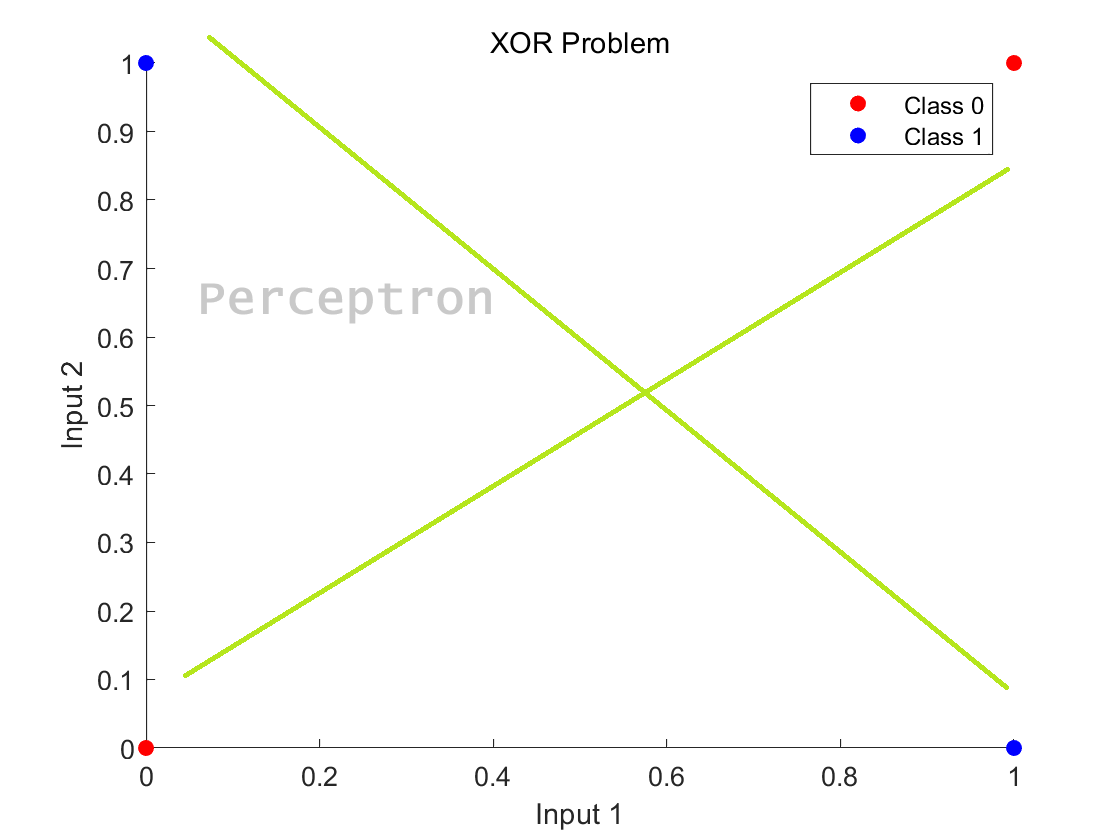
\includegraphics[width=1.0% 图片尺寸,可自行调节
        \textwidth]{XOR}% 图片名称(图片需与tex文件在同一文件夹)
        \caption{\fontsize{10pt}{15pt}\selectfont Failure on XOR}% 图例
    \end{minipage}
\end{figure}
\begin{solution}
    感知机的分类公式为$f(x)=sign(w\cdot x+b)$,只能解决严格线性可分的问题,
    但是在XOR的分类中,两个类别的点分别分布在两条对角线上,不存在可以将它们
    分开的超平面,因此无法由感知机实现分类
\end{solution}
\begin{problem}
    求证:样本集线性可分的充分必要条件是正实例点集所构成的凸壳
    与负实例点集所构成的凸壳互不相交
\end{problem}
\begin{solution}
    $\Rightarrow$:当存在超平面$H:y=w\cdot x+b$将两种实例点分开时,有:
    \begin{align}
        &w\cdot x_i+b\textgreater 0,1\leq i\leq n\\
        &w \cdot y_i+b \textless 0,1\leq i\leq n
    \end{align}
    其中$x_i$为正实例点,$y_i$为负实例点\par
    因此有:
    \begin{align}
        &w\cdot \sum_{i = 1}^{n} \lambda_i\cdot x_i +b\textgreater 0,1\leq i\leq n\\
        &w \cdot \sum_{i = 1}^{n} \lambda_i\cdot y_i+b \textless 0,1\leq i\leq n
    \end{align}
    其中$\lambda_i\geq 0$且$\sum_{i=1}^{n} \lambda_i =1$\par
    因此两个凸壳也分布在超平面的两侧,从而两个凸壳无交\par
    $\Leftarrow $:由于两个凸壳无交,并且它们分别是$\mathbb{R}^n$中的紧集和闭集,因此它们存在正距离.
    又因为二者都是闭集,因此存在取到这个最小距离的$a\in C_1,b\in C_2$.只需取二者的中垂面,即:
    \begin{align}
        H=\{x\in \mathbb{R}^n ; d(x,a)=d(x,b)\}
    \end{align}
    那么对$y\in C_1$有$d(y,a)\textless d(y,b)$,对$y\in C_2$有$d(y,a)\textgreater d(y,b)$,
    从而$H$就是所要求的超平面
\end{solution}

\end{document}
